\label{implementation}

This chapter explains implementation details of \tbas\ running on \thismachine.

\section{Keycodes}

\index{keycodes}This is a table of keycodes recognised by the LibGDX, a framework that \thismachine\ runs on.

\begin{longtable}{*{2}{m{\textwidth}}}\hline
\endfirsthead
\endhead

\endfoot
\hline
\endlastfoot
\centering
\begin{tabulary}{\textwidth}{rl}
Key & Code \\
\hline
\ttfamily{1} & 8 \\
\ttfamily{2} & 9 \\
\ttfamily{3} & 10 \\
\ttfamily{4} & 11 \\
\ttfamily{5} & 12 \\
\ttfamily{6} & 13 \\
\ttfamily{7} & 14 \\
\ttfamily{8} & 15 \\
\ttfamily{9} & 16 \\
\ttfamily{0} & 17 \\
$\hookleftarrow$ & 66 \\
\condensedfont{BkSp} & 67 \\
\condensedfont{Tab} & 61 \\
\ttfamily{`} & 68 \\
\ttfamily{'} & 75 \\
\ttfamily{;} & 43 \\
\ttfamily{,} & 55 \\
\ttfamily{.} & 56 \\
\ttfamily{/} & 76 \\
\ttfamily{[}\hspace*{0.083em} & 71 \\
\ttfamily{]}\hspace*{-0.083em} & 72 \\
\ttfamily{-} & 69 \\
\end{tabulary}
\begin{tabulary}{\textwidth}{rl}
Key & Code \\
\hline
\ttfamily{+} & 70 \\
\ttfamily{A} & 29 \\
\ttfamily{B} & 30 \\
\ttfamily{C} & 31 \\
\ttfamily{D} & 32\\
\ttfamily{E} & 33 \\
\ttfamily{F} & 34 \\
\ttfamily{G} & 35 \\
\ttfamily{H} & 36 \\
\ttfamily{I} & 37 \\
\ttfamily{J} & 38 \\
\ttfamily{K} & 39 \\
\ttfamily{L} & 40 \\
\ttfamily{M} & 41 \\
\ttfamily{N} & 42 \\
\ttfamily{O} & 43 \\
\ttfamily{P} & 44 \\
\ttfamily{Q} & 45 \\
\ttfamily{R} & 46 \\
\ttfamily{S} & 47 \\
\ttfamily{T} & 48 \\
\ttfamily{U} & 49 \\
\end{tabulary}
\begin{tabulary}{\textwidth}{rl}
Key & Code \\
\hline
\ttfamily{V} & 50 \\
\ttfamily{W} & 51 \\
\ttfamily{X} & 52 \\
\ttfamily{Y} & 53 \\
\ttfamily{Z} & 54 \\
\condensedfont{LCtrl} & 57 \\
\condensedfont{RCtrl} & 58 \\
\condensedfont{LShift} & 59 \\
\condensedfont{RShift} & 60 \\
\condensedfont{LAlt} & 129 \\
\condensedfont{RAlt} & 130 \\
$\uparrow$ & 19 \\
$\downarrow$ & 20 \\
$\leftarrow$ & 21 \\
$\rightarrow$ & 22 \\
\condensedfont{Ins} & 133 \\
\condensedfont{Del} & 112 \\
\condensedfont{PgUp} & 92 \\
\condensedfont{PgDn} & 93 \\
\condensedfont{Home} & 3 \\
\condensedfont{End} & 132 \\
F1 & 244 \\
\end{tabulary}
\begin{tabulary}{\textwidth}{rl}
Key & Code \\
\hline
F2 & 245 \\
F3 & 246 \\
F4 & 247 \\
F5 & 248 \\
F6 & 249 \\
F7 & 250 \\
F8 & 251 \\
F9 & 252 \\
F10 & 253 \\
F11 & 254 \\
\condensedfont{Num} \ttfamily{0} & 144 \\
\condensedfont{Num} \ttfamily{1} & 145 \\
\condensedfont{Num} \ttfamily{2} & 146 \\
\condensedfont{Num} \ttfamily{3} & 147 \\
\condensedfont{Num} \ttfamily{4} & 148 \\
\condensedfont{Num} \ttfamily{5} & 149 \\
\condensedfont{Num} \ttfamily{6} & 150 \\
\condensedfont{Num} \ttfamily{7} & 151 \\
\condensedfont{Num} \ttfamily{8} & 152 \\
\condensedfont{Num} \ttfamily{9} & 153 \\
\condensedfont{NumLk} & 78 \\
\ttfamily{*} & 17 \\
\end{tabulary}
\end{longtable}

Keys not listed on the table may not be available depending on the system, for example, F12 may not be recognised.

\section{Code Page}
\label{codepage}

\index{code page}By default \thismachine\ uses slightly modified version of CP-437, this is a character map of it:

{\centering
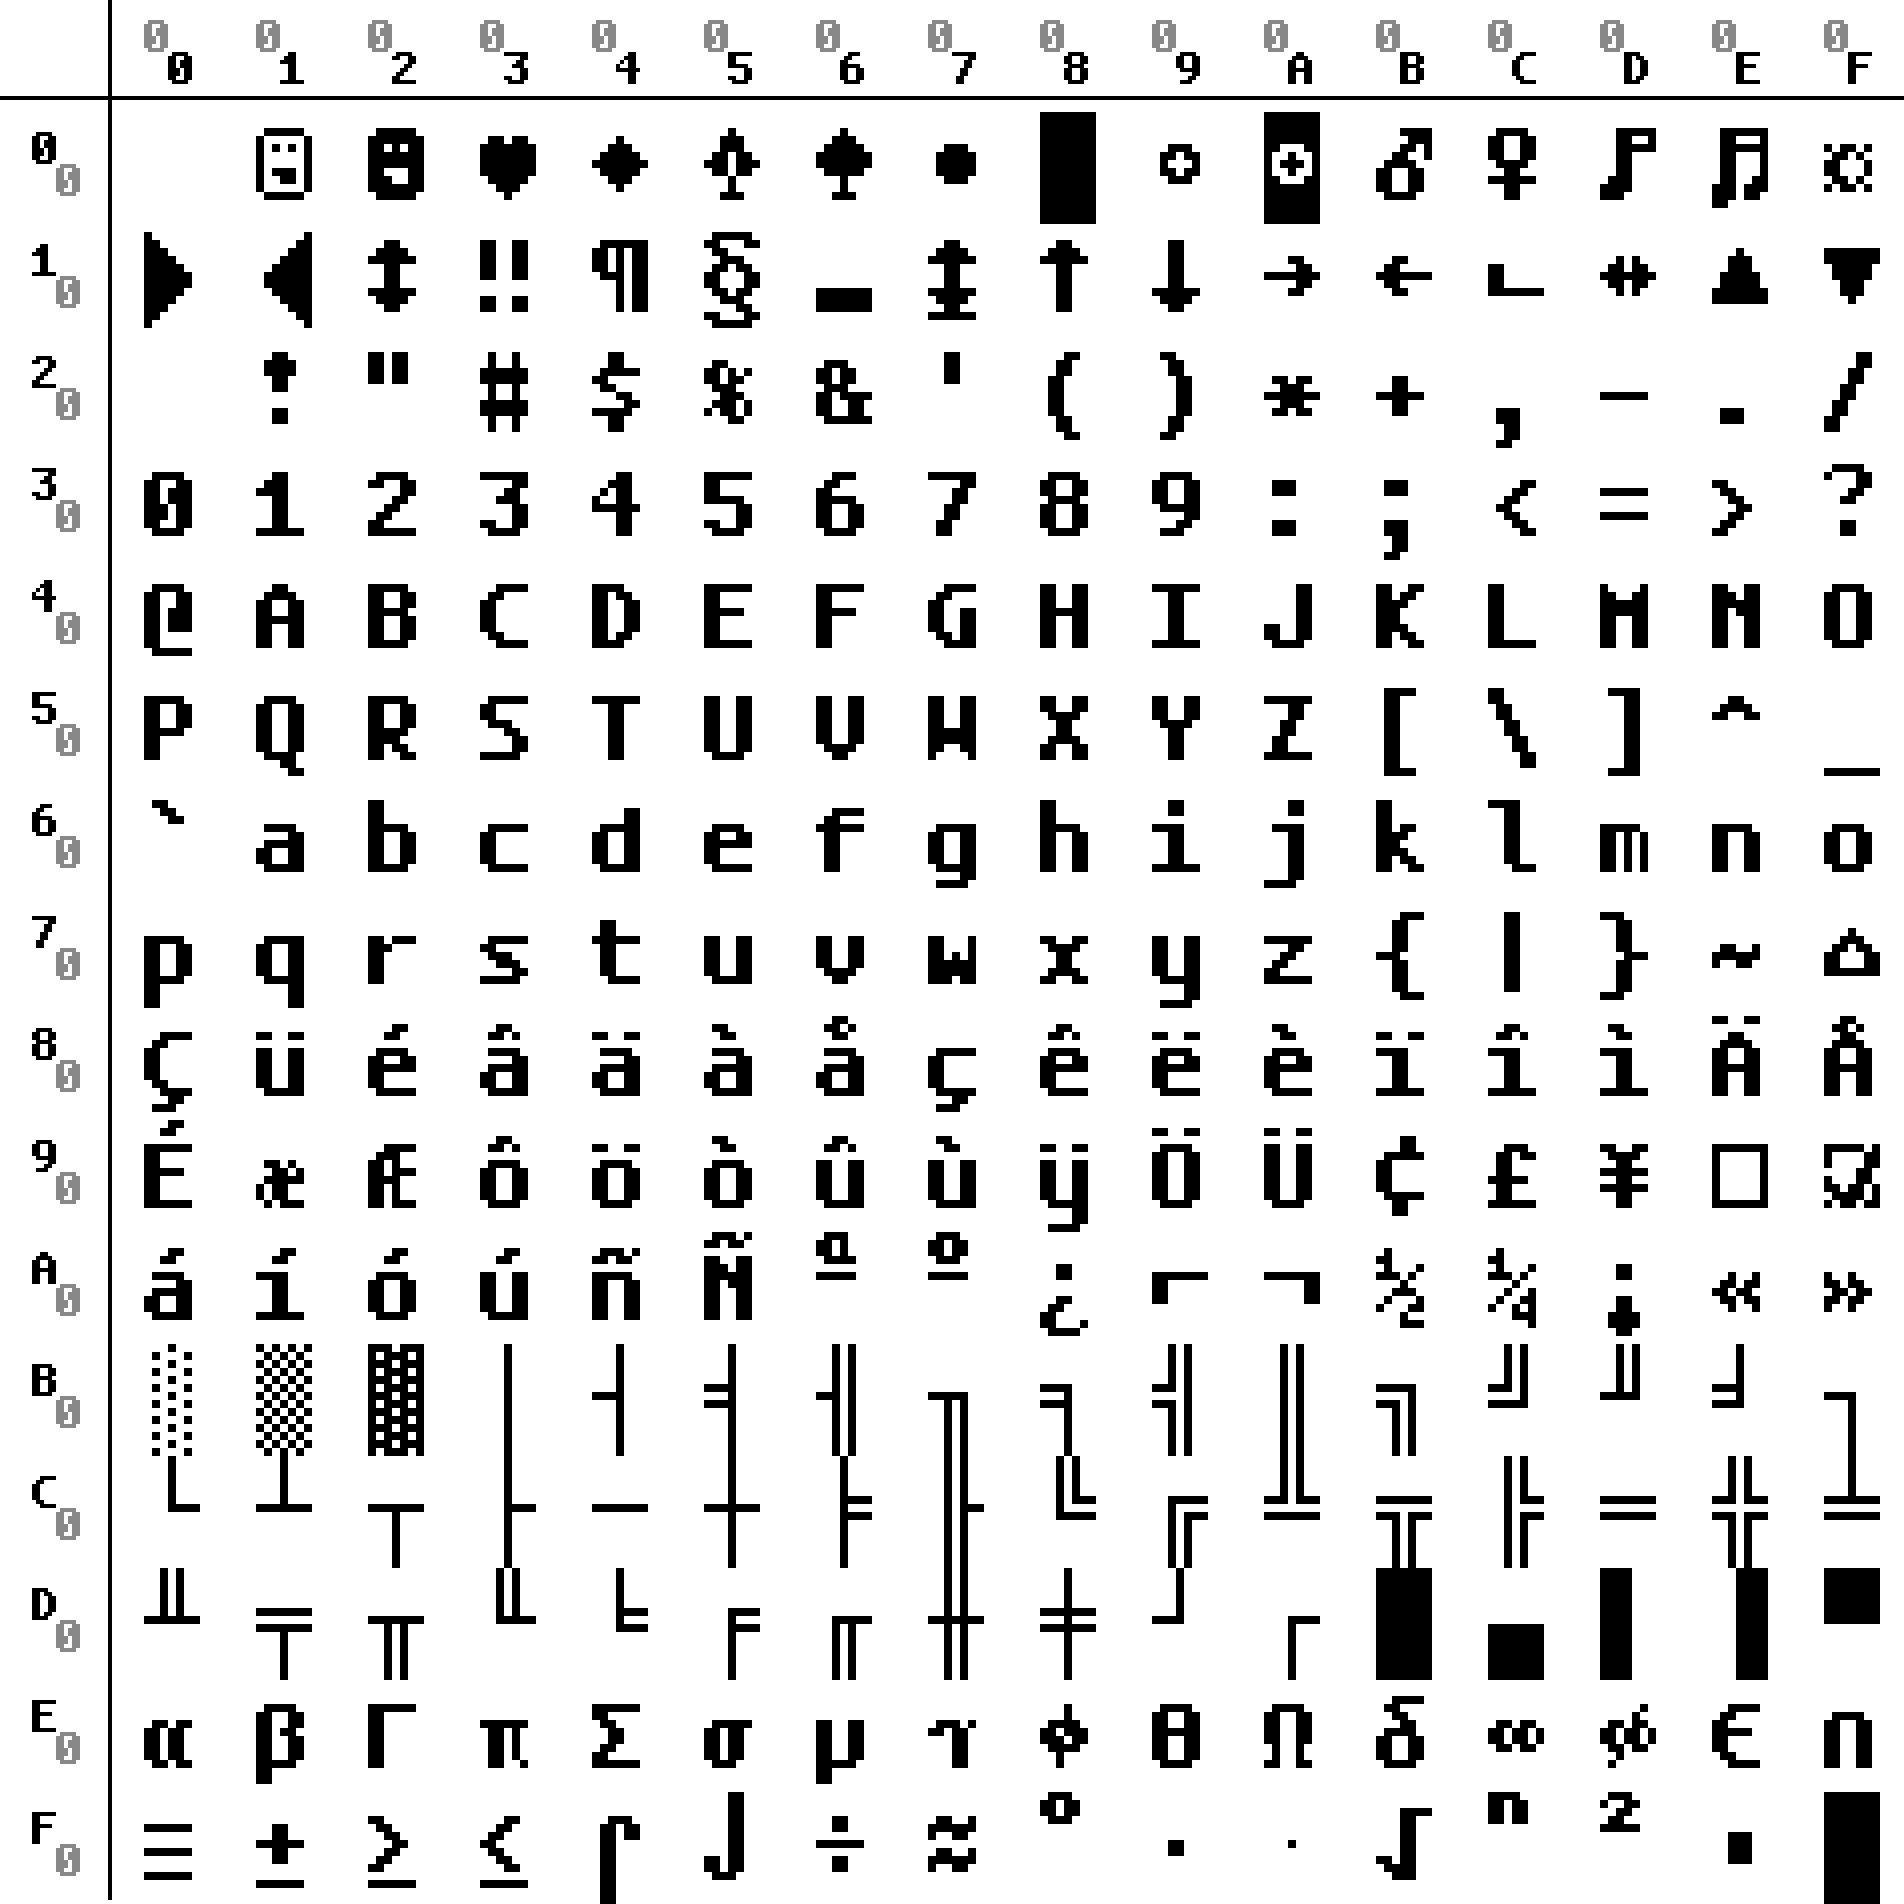
\includegraphics[width=\linewidth]{tsvmcp.png}
\captionof{figure}{\thismachine\ Character Map}
\label{fig:codepage}
}
\newpage

\section{Colour Palette}
\label{colourpalette}

\index{colour palette}By default the reference graphics adapter of the \thismachine\ uses following colour palette:

{\centering
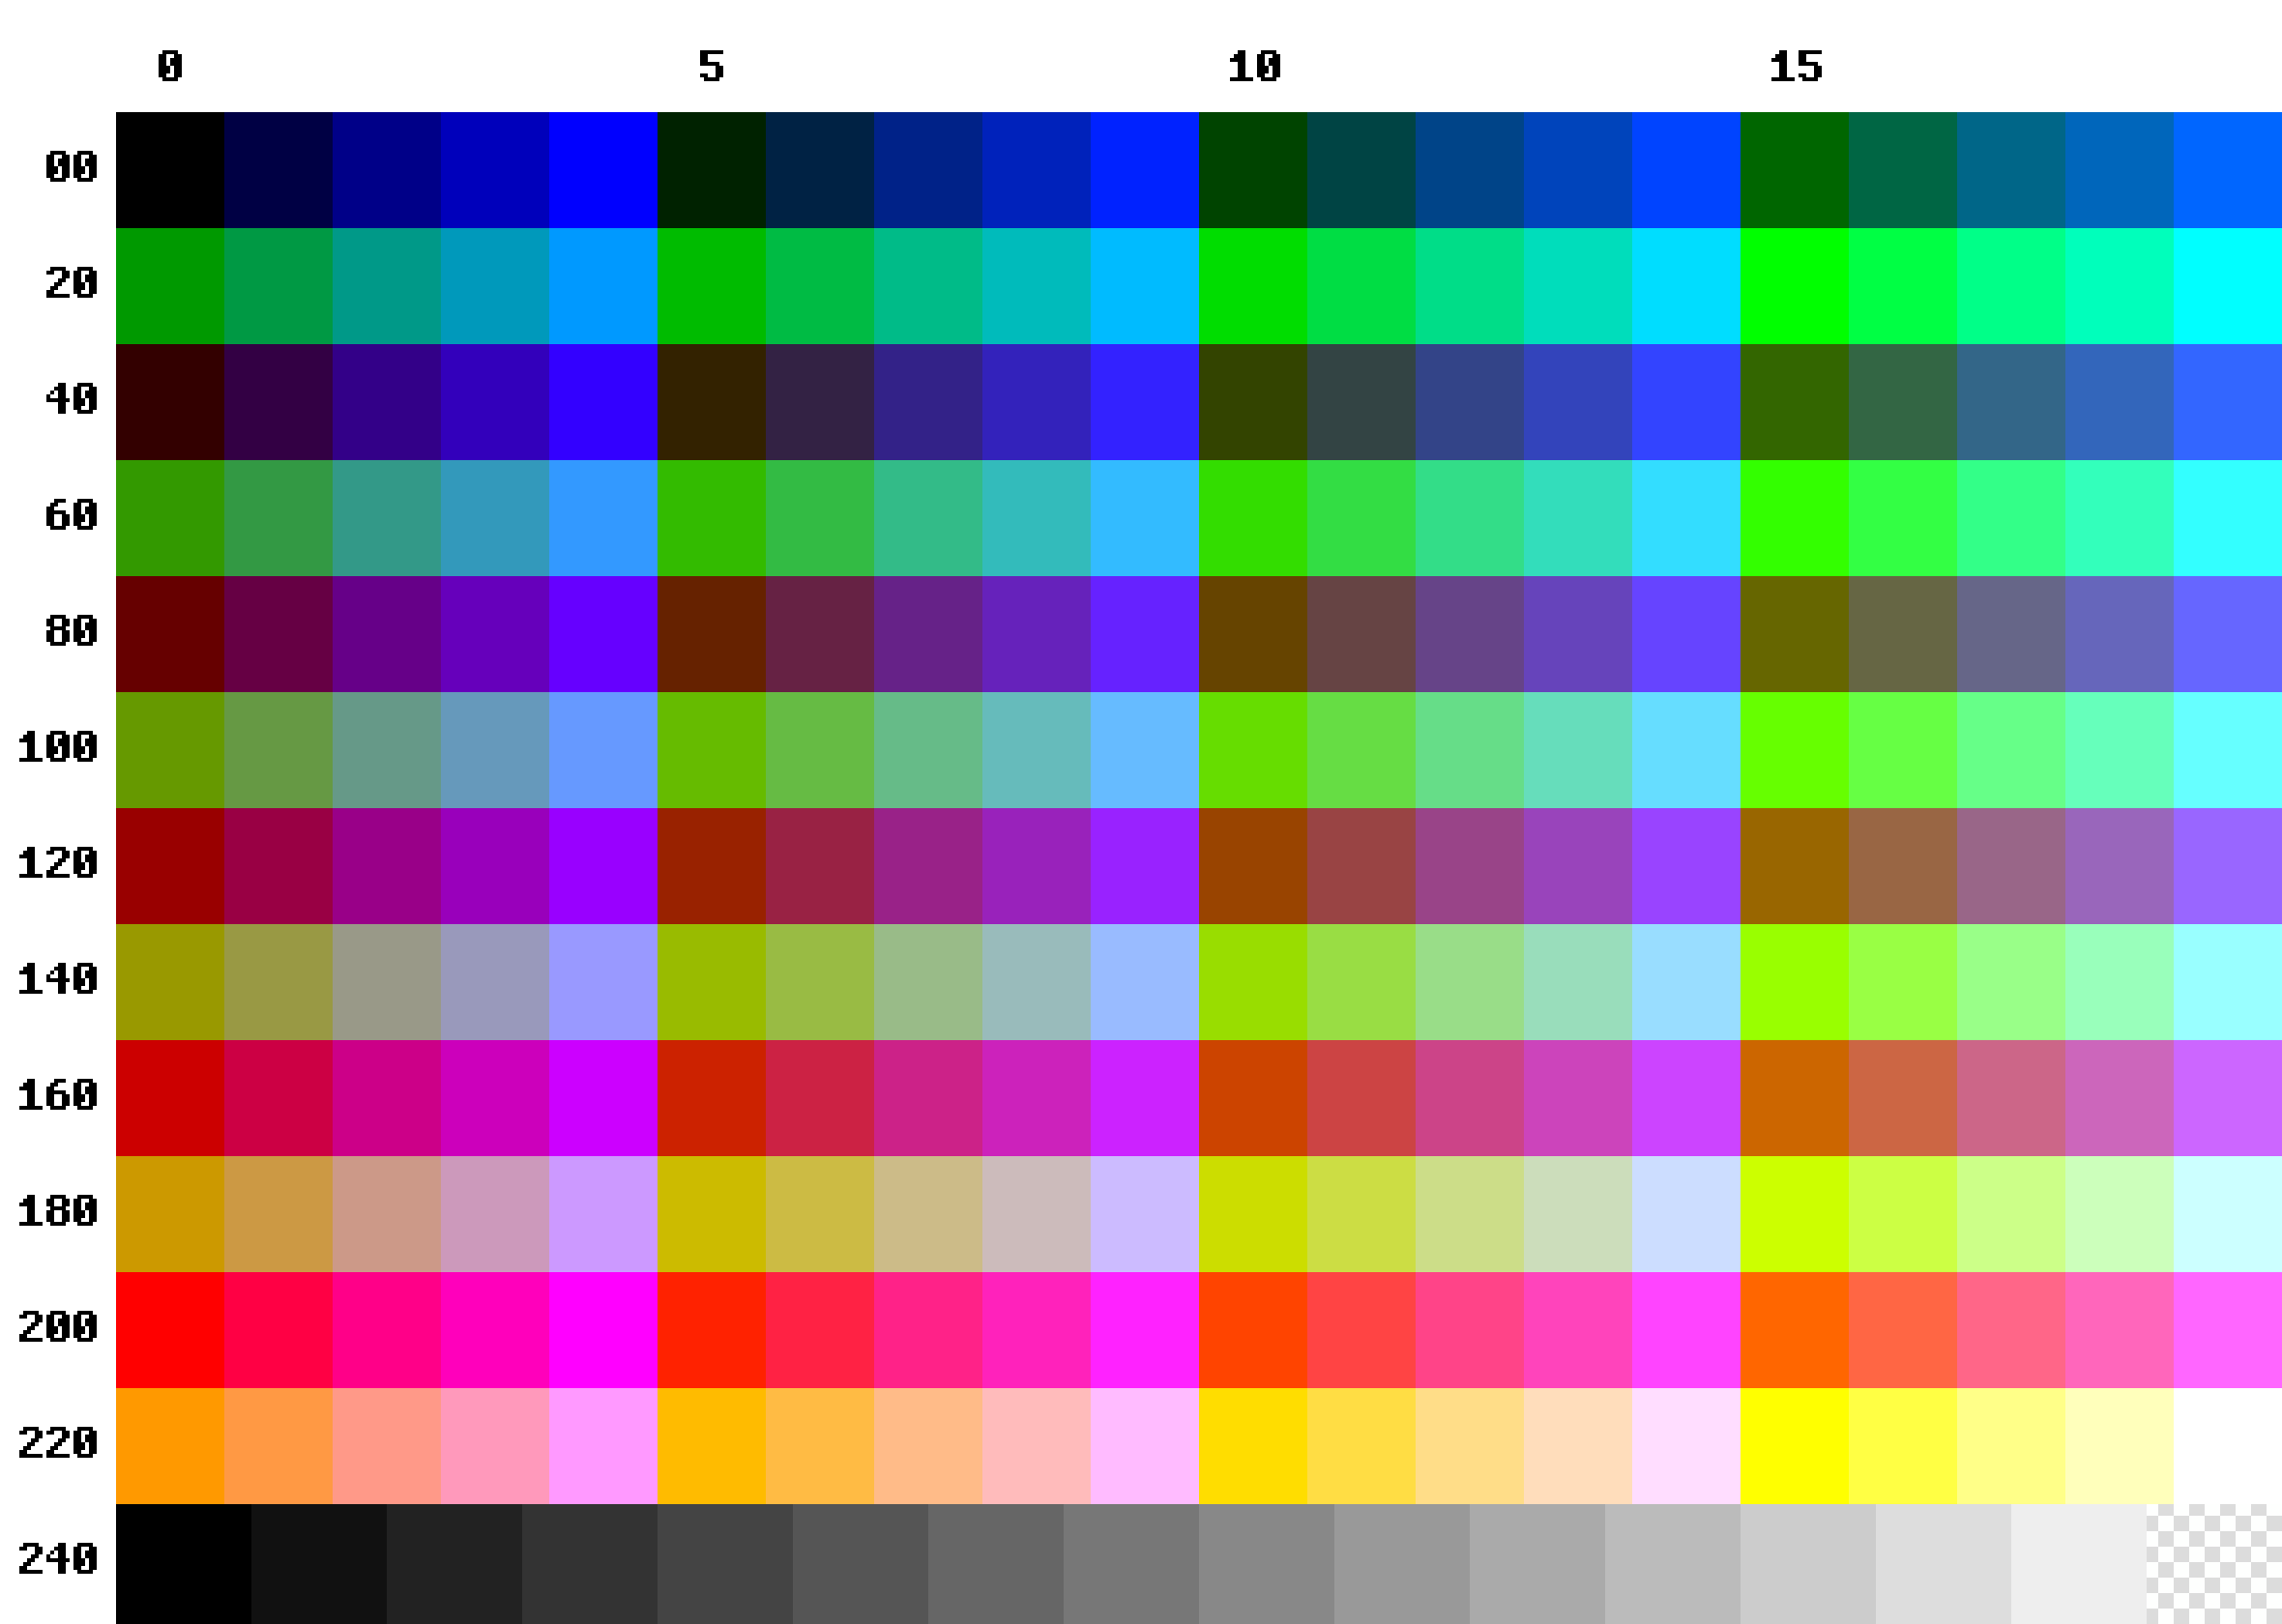
\includegraphics[width=\linewidth]{tsvmpal.png}
\captionof{figure}{\thismachine\ Colour Palette}
\label{fig:codepage}
}

{\centering
\fontsize{7pt}{0pt} % second argument is baselineskip but it's useless in table
\newlength{\extrarowheighttwo}
\setlength{\extrarowheighttwo}{\extrarowheight}
\setlength{\extrarowheight}{-0.2ex}

\begin{longtable}{*{2}{m{\textwidth}}}\hline
\endfirsthead
\endhead

\endfoot
\hline
\endlastfoot
\centering
\begin{tabulary}{\textwidth}{rl}
{\ttfamily 0} & {\ttfamily \#000F} \\
{\ttfamily 1} & {\ttfamily \#004F} \\
{\ttfamily 2} & {\ttfamily \#008F} \\
{\ttfamily 3} & {\ttfamily \#00BF} \\
{\ttfamily 4} & {\ttfamily \#00FF} \\
{\ttfamily 5} & {\ttfamily \#020F} \\
{\ttfamily 6} & {\ttfamily \#024F} \\
{\ttfamily 7} & {\ttfamily \#028F} \\
{\ttfamily 8} & {\ttfamily \#02BF} \\
{\ttfamily 9} & {\ttfamily \#02FF} \\
{\ttfamily 10} & {\ttfamily \#040F} \\
{\ttfamily 11} & {\ttfamily \#044F} \\
{\ttfamily 12} & {\ttfamily \#048F} \\
{\ttfamily 13} & {\ttfamily \#04BF} \\
{\ttfamily 14} & {\ttfamily \#04FF} \\
{\ttfamily 15} & {\ttfamily \#060F} \\
{\ttfamily 16} & {\ttfamily \#064F} \\
{\ttfamily 17} & {\ttfamily \#068F} \\
{\ttfamily 18} & {\ttfamily \#06BF} \\
{\ttfamily 19} & {\ttfamily \#06FF} \\
{\ttfamily 20} & {\ttfamily \#090F} \\
{\ttfamily 21} & {\ttfamily \#094F} \\
{\ttfamily 22} & {\ttfamily \#098F} \\
{\ttfamily 23} & {\ttfamily \#09BF} \\
{\ttfamily 24} & {\ttfamily \#09FF} \\
{\ttfamily 25} & {\ttfamily \#0B0F} \\
{\ttfamily 26} & {\ttfamily \#0B4F} \\
{\ttfamily 27} & {\ttfamily \#0B8F} \\
{\ttfamily 28} & {\ttfamily \#0BBF} \\
{\ttfamily 29} & {\ttfamily \#0BFF} \\
{\ttfamily 30} & {\ttfamily \#0D0F} \\
{\ttfamily 31} & {\ttfamily \#0D4F} \\
{\ttfamily 32} & {\ttfamily \#0D8F} \\
{\ttfamily 33} & {\ttfamily \#0DBF} \\
{\ttfamily 34} & {\ttfamily \#0DFF} \\
{\ttfamily 35} & {\ttfamily \#0F0F} \\
{\ttfamily 36} & {\ttfamily \#0F4F} \\
{\ttfamily 37} & {\ttfamily \#0F8F} \\
{\ttfamily 38} & {\ttfamily \#0FBF} \\
{\ttfamily 39} & {\ttfamily \#0FFF} \\
{\ttfamily 40} & {\ttfamily \#300F} \\
{\ttfamily 41} & {\ttfamily \#304F} \\
{\ttfamily 42} & {\ttfamily \#308F} \\
\end{tabulary}
\begin{tabulary}{\textwidth}{|rl}
{\ttfamily 43} & {\ttfamily \#30BF} \\
{\ttfamily 44} & {\ttfamily \#30FF} \\
{\ttfamily 45} & {\ttfamily \#320F} \\
{\ttfamily 46} & {\ttfamily \#324F} \\
{\ttfamily 47} & {\ttfamily \#328F} \\
{\ttfamily 48} & {\ttfamily \#32BF} \\
{\ttfamily 49} & {\ttfamily \#32FF} \\
{\ttfamily 50} & {\ttfamily \#340F} \\
{\ttfamily 51} & {\ttfamily \#344F} \\
{\ttfamily 52} & {\ttfamily \#348F} \\
{\ttfamily 53} & {\ttfamily \#34BF} \\
{\ttfamily 54} & {\ttfamily \#34FF} \\
{\ttfamily 55} & {\ttfamily \#360F} \\
{\ttfamily 56} & {\ttfamily \#364F} \\
{\ttfamily 57} & {\ttfamily \#368F} \\
{\ttfamily 58} & {\ttfamily \#36BF} \\
{\ttfamily 59} & {\ttfamily \#36FF} \\
{\ttfamily 60} & {\ttfamily \#390F} \\
{\ttfamily 61} & {\ttfamily \#394F} \\
{\ttfamily 62} & {\ttfamily \#398F} \\
{\ttfamily 63} & {\ttfamily \#39BF} \\
{\ttfamily 64} & {\ttfamily \#39FF} \\
{\ttfamily 65} & {\ttfamily \#3B0F} \\
{\ttfamily 66} & {\ttfamily \#3B4F} \\
{\ttfamily 67} & {\ttfamily \#3B8F} \\
{\ttfamily 68} & {\ttfamily \#3BBF} \\
{\ttfamily 69} & {\ttfamily \#3BFF} \\
{\ttfamily 70} & {\ttfamily \#3D0F} \\
{\ttfamily 71} & {\ttfamily \#3D4F} \\
{\ttfamily 72} & {\ttfamily \#3D8F} \\
{\ttfamily 73} & {\ttfamily \#3DBF} \\
{\ttfamily 74} & {\ttfamily \#3DFF} \\
{\ttfamily 75} & {\ttfamily \#3F0F} \\
{\ttfamily 76} & {\ttfamily \#3F4F} \\
{\ttfamily 77} & {\ttfamily \#3F8F} \\
{\ttfamily 78} & {\ttfamily \#3FBF} \\
{\ttfamily 79} & {\ttfamily \#3FFF} \\
{\ttfamily 80} & {\ttfamily \#600F} \\
{\ttfamily 81} & {\ttfamily \#604F} \\
{\ttfamily 82} & {\ttfamily \#608F} \\
{\ttfamily 83} & {\ttfamily \#60BF} \\
{\ttfamily 84} & {\ttfamily \#60FF} \\
{\ttfamily 85} & {\ttfamily \#620F} \\
\end{tabulary}
\begin{tabulary}{\textwidth}{|rl}
{\ttfamily 86} & {\ttfamily \#624F} \\
{\ttfamily 87} & {\ttfamily \#628F} \\
{\ttfamily 88} & {\ttfamily \#62BF} \\
{\ttfamily 89} & {\ttfamily \#62FF} \\
{\ttfamily 90} & {\ttfamily \#640F} \\
{\ttfamily 91} & {\ttfamily \#644F} \\
{\ttfamily 92} & {\ttfamily \#648F} \\
{\ttfamily 93} & {\ttfamily \#64BF} \\
{\ttfamily 94} & {\ttfamily \#64FF} \\
{\ttfamily 95} & {\ttfamily \#660F} \\
{\ttfamily 96} & {\ttfamily \#664F} \\
{\ttfamily 97} & {\ttfamily \#668F} \\
{\ttfamily 98} & {\ttfamily \#66BF} \\
{\ttfamily 99} & {\ttfamily \#66FF} \\
{\ttfamily 100} & {\ttfamily \#690F} \\
{\ttfamily 101} & {\ttfamily \#694F} \\
{\ttfamily 102} & {\ttfamily \#698F} \\
{\ttfamily 103} & {\ttfamily \#69BF} \\
{\ttfamily 104} & {\ttfamily \#69FF} \\
{\ttfamily 105} & {\ttfamily \#6B0F} \\
{\ttfamily 106} & {\ttfamily \#6B4F} \\
{\ttfamily 107} & {\ttfamily \#6B8F} \\
{\ttfamily 108} & {\ttfamily \#6BBF} \\
{\ttfamily 109} & {\ttfamily \#6BFF} \\
{\ttfamily 110} & {\ttfamily \#6D0F} \\
{\ttfamily 111} & {\ttfamily \#6D4F} \\
{\ttfamily 112} & {\ttfamily \#6D8F} \\
{\ttfamily 113} & {\ttfamily \#6DBF} \\
{\ttfamily 114} & {\ttfamily \#6DFF} \\
{\ttfamily 115} & {\ttfamily \#6F0F} \\
{\ttfamily 116} & {\ttfamily \#6F4F} \\
{\ttfamily 117} & {\ttfamily \#6F8F} \\
{\ttfamily 118} & {\ttfamily \#6FBF} \\
{\ttfamily 119} & {\ttfamily \#6FFF} \\
{\ttfamily 120} & {\ttfamily \#900F} \\
{\ttfamily 121} & {\ttfamily \#904F} \\
{\ttfamily 122} & {\ttfamily \#908F} \\
{\ttfamily 123} & {\ttfamily \#90BF} \\
{\ttfamily 124} & {\ttfamily \#90FF} \\
{\ttfamily 125} & {\ttfamily \#920F} \\
{\ttfamily 126} & {\ttfamily \#924F} \\
{\ttfamily 127} & {\ttfamily \#928F} \\
{\ttfamily 128} & {\ttfamily \#92BF} \\
\end{tabulary}
\begin{tabulary}{\textwidth}{|rl}
{\ttfamily 129} & {\ttfamily \#92FF} \\
{\ttfamily 130} & {\ttfamily \#940F} \\
{\ttfamily 131} & {\ttfamily \#944F} \\
{\ttfamily 132} & {\ttfamily \#948F} \\
{\ttfamily 133} & {\ttfamily \#94BF} \\
{\ttfamily 134} & {\ttfamily \#94FF} \\
{\ttfamily 135} & {\ttfamily \#960F} \\
{\ttfamily 136} & {\ttfamily \#964F} \\
{\ttfamily 137} & {\ttfamily \#968F} \\
{\ttfamily 138} & {\ttfamily \#96BF} \\
{\ttfamily 139} & {\ttfamily \#96FF} \\
{\ttfamily 140} & {\ttfamily \#990F} \\
{\ttfamily 141} & {\ttfamily \#994F} \\
{\ttfamily 142} & {\ttfamily \#998F} \\
{\ttfamily 143} & {\ttfamily \#99BF} \\
{\ttfamily 144} & {\ttfamily \#99FF} \\
{\ttfamily 145} & {\ttfamily \#9B0F} \\
{\ttfamily 146} & {\ttfamily \#9B4F} \\
{\ttfamily 147} & {\ttfamily \#9B8F} \\
{\ttfamily 148} & {\ttfamily \#9BBF} \\
{\ttfamily 149} & {\ttfamily \#9BFF} \\
{\ttfamily 150} & {\ttfamily \#9D0F} \\
{\ttfamily 151} & {\ttfamily \#9D4F} \\
{\ttfamily 152} & {\ttfamily \#9D8F} \\
{\ttfamily 153} & {\ttfamily \#9DBF} \\
{\ttfamily 154} & {\ttfamily \#9DFF} \\
{\ttfamily 155} & {\ttfamily \#9F0F} \\
{\ttfamily 156} & {\ttfamily \#9F4F} \\
{\ttfamily 157} & {\ttfamily \#9F8F} \\
{\ttfamily 158} & {\ttfamily \#9FBF} \\
{\ttfamily 159} & {\ttfamily \#9FFF} \\
{\ttfamily 160} & {\ttfamily \#C00F} \\
{\ttfamily 161} & {\ttfamily \#C04F} \\
{\ttfamily 162} & {\ttfamily \#C08F} \\
{\ttfamily 163} & {\ttfamily \#C0BF} \\
{\ttfamily 164} & {\ttfamily \#C0FF} \\
{\ttfamily 165} & {\ttfamily \#C20F} \\
{\ttfamily 166} & {\ttfamily \#C24F} \\
{\ttfamily 167} & {\ttfamily \#C28F} \\
{\ttfamily 168} & {\ttfamily \#C2BF} \\
{\ttfamily 169} & {\ttfamily \#C2FF} \\
{\ttfamily 170} & {\ttfamily \#C40F} \\
{\ttfamily 171} & {\ttfamily \#C44F} \\
\end{tabulary}
\begin{tabulary}{\textwidth}{|rl}
{\ttfamily 172} & {\ttfamily \#C48F} \\
{\ttfamily 173} & {\ttfamily \#C4BF} \\
{\ttfamily 174} & {\ttfamily \#C4FF} \\
{\ttfamily 175} & {\ttfamily \#C60F} \\
{\ttfamily 176} & {\ttfamily \#C64F} \\
{\ttfamily 177} & {\ttfamily \#C68F} \\
{\ttfamily 178} & {\ttfamily \#C6BF} \\
{\ttfamily 179} & {\ttfamily \#C6FF} \\
{\ttfamily 180} & {\ttfamily \#C90F} \\
{\ttfamily 181} & {\ttfamily \#C94F} \\
{\ttfamily 182} & {\ttfamily \#C98F} \\
{\ttfamily 183} & {\ttfamily \#C9BF} \\
{\ttfamily 184} & {\ttfamily \#C9FF} \\
{\ttfamily 185} & {\ttfamily \#CB0F} \\
{\ttfamily 186} & {\ttfamily \#CB4F} \\
{\ttfamily 187} & {\ttfamily \#CB8F} \\
{\ttfamily 188} & {\ttfamily \#CBBF} \\
{\ttfamily 189} & {\ttfamily \#CBFF} \\
{\ttfamily 190} & {\ttfamily \#CD0F} \\
{\ttfamily 191} & {\ttfamily \#CD4F} \\
{\ttfamily 192} & {\ttfamily \#CD8F} \\
{\ttfamily 193} & {\ttfamily \#CDBF} \\
{\ttfamily 194} & {\ttfamily \#CDFF} \\
{\ttfamily 195} & {\ttfamily \#CF0F} \\
{\ttfamily 196} & {\ttfamily \#CF4F} \\
{\ttfamily 197} & {\ttfamily \#CF8F} \\
{\ttfamily 198} & {\ttfamily \#CFBF} \\
{\ttfamily 199} & {\ttfamily \#CFFF} \\
{\ttfamily 200} & {\ttfamily \#F00F} \\
{\ttfamily 201} & {\ttfamily \#F04F} \\
{\ttfamily 202} & {\ttfamily \#F08F} \\
{\ttfamily 203} & {\ttfamily \#F0BF} \\
{\ttfamily 204} & {\ttfamily \#F0FF} \\
{\ttfamily 205} & {\ttfamily \#F20F} \\
{\ttfamily 206} & {\ttfamily \#F24F} \\
{\ttfamily 207} & {\ttfamily \#F28F} \\
{\ttfamily 208} & {\ttfamily \#F2BF} \\
{\ttfamily 209} & {\ttfamily \#F2FF} \\
{\ttfamily 210} & {\ttfamily \#F40F} \\
{\ttfamily 211} & {\ttfamily \#F44F} \\
{\ttfamily 212} & {\ttfamily \#F48F} \\
{\ttfamily 213} & {\ttfamily \#F4BF} \\
{\ttfamily 214} & {\ttfamily \#F4FF} \\
\end{tabulary}
\begin{tabulary}{\textwidth}{|rl}
{\ttfamily 215} & {\ttfamily \#F60F} \\
{\ttfamily 216} & {\ttfamily \#F64F} \\
{\ttfamily 217} & {\ttfamily \#F68F} \\
{\ttfamily 218} & {\ttfamily \#F6BF} \\
{\ttfamily 219} & {\ttfamily \#F6FF} \\
{\ttfamily 220} & {\ttfamily \#F90F} \\
{\ttfamily 221} & {\ttfamily \#F94F} \\
{\ttfamily 222} & {\ttfamily \#F98F} \\
{\ttfamily 223} & {\ttfamily \#F9BF} \\
{\ttfamily 224} & {\ttfamily \#F9FF} \\
{\ttfamily 225} & {\ttfamily \#FB0F} \\
{\ttfamily 226} & {\ttfamily \#FB4F} \\
{\ttfamily 227} & {\ttfamily \#FB8F} \\
{\ttfamily 228} & {\ttfamily \#FBBF} \\
{\ttfamily 229} & {\ttfamily \#FBFF} \\
{\ttfamily 230} & {\ttfamily \#FD0F} \\
{\ttfamily 231} & {\ttfamily \#FD4F} \\
{\ttfamily 232} & {\ttfamily \#FD8F} \\
{\ttfamily 233} & {\ttfamily \#FDBF} \\
{\ttfamily 234} & {\ttfamily \#FDFF} \\
{\ttfamily 235} & {\ttfamily \#FF0F} \\
{\ttfamily 236} & {\ttfamily \#FF4F} \\
{\ttfamily 237} & {\ttfamily \#FF8F} \\
{\ttfamily 238} & {\ttfamily \#FFBF} \\
{\ttfamily 239} & {\ttfamily \#FFFF} \\
{\ttfamily 240} & {\ttfamily \#000F} \\
{\ttfamily 241} & {\ttfamily \#111F} \\
{\ttfamily 242} & {\ttfamily \#222F} \\
{\ttfamily 243} & {\ttfamily \#333F} \\
{\ttfamily 244} & {\ttfamily \#444F} \\
{\ttfamily 245} & {\ttfamily \#555F} \\
{\ttfamily 246} & {\ttfamily \#666F} \\
{\ttfamily 247} & {\ttfamily \#777F} \\
{\ttfamily 248} & {\ttfamily \#888F} \\
{\ttfamily 249} & {\ttfamily \#999F} \\
{\ttfamily 250} & {\ttfamily \#AAAF} \\
{\ttfamily 251} & {\ttfamily \#BBBF} \\
{\ttfamily 252} & {\ttfamily \#CCCF} \\
{\ttfamily 253} & {\ttfamily \#DDDF} \\
{\ttfamily 254} & {\ttfamily \#EEEF} \\
{\ttfamily 255} & {\ttfamily \#0000} \\
\, & \, \\
\, & \, \\
\end{tabulary}
\end{longtable}

\captionof{table}{Index--RGBA Table of the Colour Palette}
}

\setlength{\extrarowheight}{\extrarowheighttwo}

\section{MMIO}

\label{mmio}\index{mmio}Some parts of the memory address are mapped to some devices. This section will describe useful memory addresses that can be \code{POKE}d.

For more detailed documentation, refer to the manuals for \thismachine.

\begin{tabulary}{\textwidth}{Rl}
Address & Description \\
\hline
-1048577..-1299456 & Screen Buffer \\
-1299457 & Screen Background RED \\
-1299458 & Screen Background GREEN \\
-1299459 & Screen Background BLUE \\
-1302527 & Text Cursor Position in $row \times 32 + col$ \\
-1302529 & Text Foreground Colours \\
-1305089 & Text Background Colours \\
-1307649 & Text Buffer \\
-1310209 & Palettes in This Pattern: {\ttfamily 0b RRRR GGGG; 0b BBBB AAAA} \\
\end{tabulary}
